\documentclass[10pt]{article}

\usepackage[a4paper,
            bindingoffset=0.2in,
            left=1in,
            right=1in,
            top=1in,
            bottom=1in,
            footskip=.25in]{geometry}
\usepackage{mathtools}
\usepackage{amsmath}
\usepackage{amssymb}
\usepackage{enumitem}
\usepackage{environ}
\usepackage{tikz}
\usepackage{graphicx}
\graphicspath{ {./images/} }

\NewEnviron{suneq}{%
\begin{equation*}\begin{split}
  \BODY
\end{split}\end{equation*}
}

\DeclareMathOperator{\Prob}{\text{P}}
\DeclareMathOperator{\E}{\text{E}}
\DeclareMathOperator{\Var}{\text{Var}}

\DeclarePairedDelimiter\abs{\lvert}{\rvert}%
\DeclarePairedDelimiter\norm{\lVert}{\rVert}%

\newcommand*{\Perm}[2]{{}^{#1}\!P_{#2}}%
\newcommand*{\Comb}[2]{{}^{#1}C_{#2}}%

\begin{document}

\title{Modelling Uncertainty 1D Project}
\author{\b{SC06 Group 4}\\Guo Ziniu, Yeoh Siew Ning, Devon Cheng, Yong Zheng Yew}


\maketitle
\section*{Q0.}
\begin{center}
    \begin{tabular}{ c c }
        Yong Zheng Yew & 1005155 \\ 
        Yeoh Siew Ning & 1005471 \\  
        Devon Cheng & 1005215 \\
        Guo Ziniu & 1004890 \\
        Yeo Kai Wen & 1005291
    \end{tabular}
\end{center}
\begin{suneq}
    p_0 &= \frac{\frac{1005155+1005471+1005215+1004890+1005291}{5}-10^6}{10^4} \\
    &= 0.52044
\end{suneq}
\section*{Q1.}
\subsection*{a)}
\begin{suneq}
    F(n,m,p) = \sum_{k=0}^{m-1}\Comb{n-1+k}{k}\cdot p^{n}\left(1-p\right)^{k}
\end{suneq}
\subsection*{b)}
\begin{suneq}
    F(8,10,p_0) = 0.743459444891
\end{suneq}
\section*{Q2.}
\subsection*{a)}
\subsubsection*{}
Claim 1: Let points scored by $A$ and $B$ be $S_A$ and $S_B$ respectively.

The extended game's bounding condition is $S_A+S_B=n+m-1$. The win condition for $A$ in the extended game is $S_A\ge n$, which implies $S_B\le m-1<m$; similarly for $B$, it is $S_B\ge m\implies S_A\le n-1<n$. The order of scoring points does not matter.

By contrast, in the original game, the win condition does sometimes depend on the order of who wins their target number of points first. However, when we limit $S_A+S_B=n+m-1$, as long as in the end, $S_A\ge n$, we know that $S_B\le m-1<m$, and so $A$ must have reached $n$ at some point, while $B$ never could have, and thus regardless of order, $A$ must have won under the original game's rules as well (and vice versa for $B$). \textbf{Thus, if the extended game is won, the original game must be won.}

In a way, if the two players had been playing under the original game's rules, it would be as if, although $A$ might have possibly won halfway, they still kept playing rounds until $S_A+S_B=n+m-1$, even though under such circumstances, $B$ had no hope of winning and it would not affect the outcome, and the maximum points $B$ could score would still be less than $m$. \textbf{From this, we can see that if the original game is won, the extended game must be won.}

Therefore, the original game is won if and only if the extended game is won, and vice versa; i.e. they are equivalent.
\subsubsection*{}
Claim 2:

By definition, $F(n,m,p)$ is the probability that $A$ wins the original game. Also, in proving Claim 1, we have shown the two games to be equivalent. Therefore, $F(n,m,p)$ is also the probability that $A$ wins the extended game.
\subsection*{b)}
\begin{suneq}
    F(n,m,p) = \sum_{k=n}^{n+m-1}\Comb{n+m-1}{k}\cdot p^{k}\left(1-p\right)^{\left(n+m-1-k\right)}
\end{suneq}
\section*{Q3.}
\subsection*{a)}
Let $G$ represent the event of player $A$ eventually winning the entire game, where the game in question has so far only progressed until a particular round such that $A$ and $B$ need $n$ resp. $m$ more rounds to win (or more concisely, such that $P(G)=F(n,m,p)$). Let $R$ represent the event of a player winning that particular round. According to the rules of the game, at each round, either A or B must win. Therefore, $R$ partitions the sample space between two disjoint events:
\begin{suneq}
    R = \{R_A, R_B\}
\end{suneq}
Where $R_A$ and $R_B$ represent the events of player $A$ resp. $B$ winning that round. This is because there is no way for a round to be won by both players at once (disjoint), nor can any round have any outcome other than either $A$ or $B$ winning it (partitioning).\\\\According to the law of total probability:
\begin{suneq}
    P(G) &= \sum_n P(G\cap R_n)
\end{suneq}
By Bayes' Law,
\begin{suneq}
    P(G) &= \sum_n P(G|R_n)P(R_n)\\
    &= P(G|R_A)P(R_A) + P(G|R_B)P(R_B)
\end{suneq}
We know that $P(R_A)=p$ and $P(R_B)=(1-p)$ by definition. Also, $P(G|R_A)$ and $P(G|R_B)$ respectively are the events that player $A$ eventually wins the whole game, given that player $A$ resp. $B$ wins that particular round. As shown in Question 1b), we can determine $P(G|R_A) = F(n-1,m,p)$ and $P(G|R_B) = F(n,m-1,p)$. This is because the probability of player $A$ winning a particular game can be calculated entirely from the current gamestate, and does not depend on history of past gamestates. Therefore, continuing from above, we find that:
\begin{suneq}
    P(G) &= F(n,m,p)\\
    &= p\cdot F(n-1,m,p) + (1-p)\cdot F(n,m-1,p)\\
\end{suneq}
Finally, we note that when $A$ has no more points left to win while $B$ still does, then $A$ has just won by definition; so $P(G)=F(0,m,p)=1$. Similarly, when $B$ has no more points left to win while $A$ still does, $B$ has won, meaning $A$ has lost; thus $P(G)=F(n,0,p)=0$. Thus, we have established our base cases for a recursive solution to $F(n,m,p)$:
\begin{suneq}
    F(0,m,p) &= 1 \\
    F(n,0,p) &= 0
\end{suneq}

\subsection*{b)}
Refer to Excel.

\section*{Q4.}
Let $X_{player}$ be a random variable representing the number of turns that the game ends at (inclusive), with a win for that player.
\begin{suneq}
    P(X_A = x) &= \Comb{x-1}{x-4}\cdot p^{4}\left(1-p\right)^{\left(x-4\right)}\\
    P(X_B = x) &= \Comb{x-1}{x-4}\cdot p^{\left(x-4\right)}\left(1-p\right)^{4}\\
    X &= X_A + X_B
\end{suneq}
Let $X$ be a random variable representing the number of turns that the game ends at (inclusive), with a win for player A OR B. Since $X_A$ and $X_B$ are disjoint (Players A and B cannot both win at the same time),\\
\begin{suneq}
    P(X = x) &= P((X_A = x) \cup (X_B = x))\\
    &= P(X_A = x) + P(X_B = x)\\
    &= \Comb{x-1}{x-4}\cdot\left(p^{4}\left(1-p\right)^{\left(x-4\right)}+p^{\left(x-4\right)}\left(1-p\right)^{4}\right)
\end{suneq}

\begin{center}
    \begin{tabular}{ c || c | c | c | c }
        $x$ & 4 & 5 & 6 & 7\\
        \hline
        $P(X=x)$ & 0.126253729903 & 0.250833492582 & 0.311976886701 & 0.310935890814
    \end{tabular}
\end{center}
From the above, we can calculate that
\begin{suneq}
    E(X) &= 4\left(0.126253729903\right)\ +\ 5\left(0.250833492582\right)\ +\ 6\left(0.311976886701\right)\ +\ 7\left(0.310935890814\right)\\
    &= 5.81\text{ (to 3 s.f.)}
\end{suneq}

\section*{Q5.}
\begin{suneq}
    X&\sim\text{Binomial}(2n-1,p)\\
    \therefore E(X) = (2n-1)p,\quad\Var(X) &= (2n-1)p(1-p),\quad\sigma(X) = \sqrt{\Var(X)} = \sqrt{(2n-1)p(1-p)}\\
    \text{Distance }D\text{ between }n\text{ and }E(X) &=\frac{n-E(X)}{\sigma(X)} = \abs{\frac{n-(2n-1)p}{\sqrt{(2n-1)p(1-p)}}}\\
    &=\abs{\frac{n(1-2p)+p}{\sqrt{(2n-1)p(1-p)}}}\\
    &= \abs{\frac{n(1-2p)}{\sqrt{(2n-1)p(1-p)}} + \frac{p}{\sqrt{(2n-1)p(1-p)}}}\\
    \text{As }n\text{ tends to infinity,} & \frac{p}{\sqrt{(2n-1)p(1-p)}}\to 0\\
    \therefore D&\to\abs{\frac{n(1-2p)}{\sqrt{(2n-1)p(1-p)}}} = \abs{\frac{n(2p-1)}{\sqrt{(2n-1)p(1-p)}}}\\
    &= \abs{n\cdot\frac{(2p-1)}{\sqrt{(2n-1)p(1-p)}}}
\end{suneq}

Since $\frac{(2p-1)}{\sqrt{(2n-1)p(1-p)}}$ is always positive for $0.5<p<1$, we see that, as $n$ increases, $D$ increases.

\subsection*{b)}
From a picture, we can see that $E(X)$ is to the right of $n$. Since the distance $D$ between the two is increasing, $E(X)$ is getting further away from $n$. In plain English, this means that the amount of rounds player A is expected to win is increasing faster than the minimum amount of rounds player A has to win n order to win the game. Therefore, as $n$ increases, the probability that player A will win the game increases.

\section*{Q6.}
\begin{center}
    Game State Space Diagram:\\
    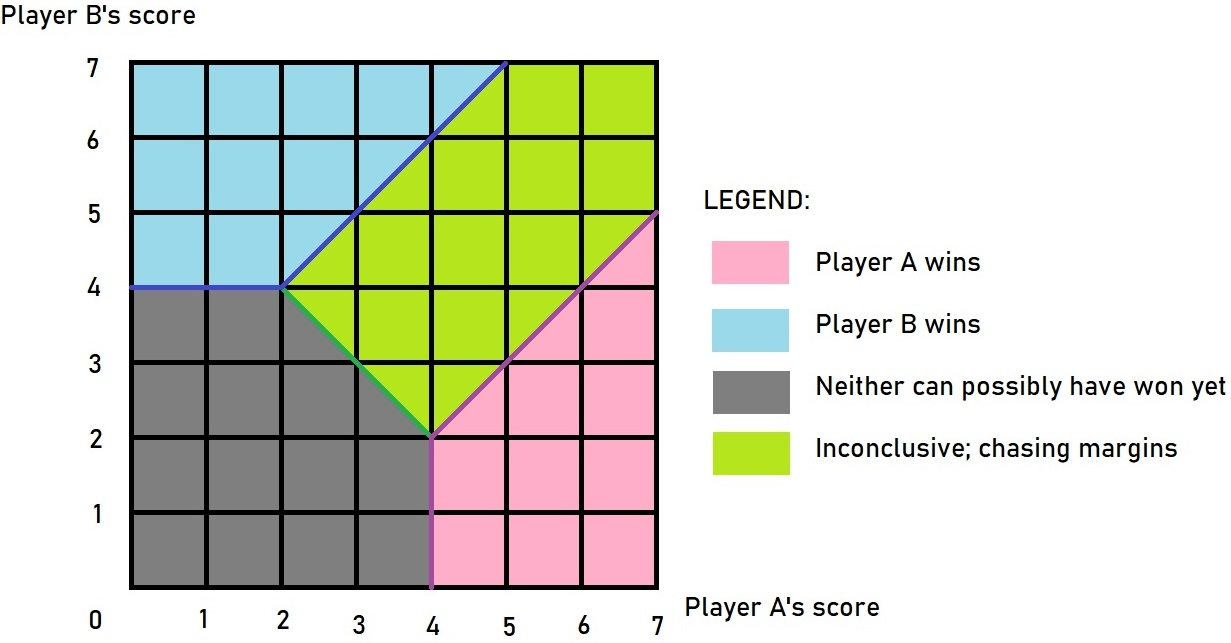
\includegraphics[width=10cm]{GameSpaceDiagram.jpg}\\
\end{center}
Probability of player A winning 4 points and player B winning $k\le2$ points (so player A wins immediately):
\begin{suneq}
    \sum_{k=0}^{2}\Comb{3+k}{3}\cdot p^{4}\left(1-p\right)^{k}
\end{suneq}
Probability of both players A and B winning 3 points each:
\begin{suneq}
    \Comb{3+3}{3}\cdot p_0^3(1-p_0)^3
\end{suneq}
If both players are at 3 points each, what matters from then on is only the margin between the two. For each round, the probabilities of:
\begin{itemize}
    \item A wins: $p_0^2$
    \item B wins: $(1-p_0)^2$
    \item Inconclusive: $\Comb{2}{1}\cdot p_0^1(1-p_0)^1 = 2p_0(1-p_0)$
\end{itemize}
Therefore, the probability of player A winning the game under these circumstances is:
\begin{suneq}
    p_0^2 + 2p_0(1-p_0)p_0^2 + [2p_0(1-p_0)]^2p_0^2 + [2p_0(1-p_0)]^3p_0^2\cdots &= p_0^2 \sum_{i=0}^{\infty}(2p_0(1-p_0))^i\\
    &= \frac{p_0^2}{1-2p_0+2p_0^2}
\end{suneq}
Therefore, the total probability that player A wins the game is:
\begin{suneq}
    \sum_{k=0}^{2}\Comb{3+k}{3}\cdot p^{4}\left(1-p\right)^{k} + \Comb{3+3}{3}\cdot p_0^3(1-p_0)^3\cdot \frac{p_0^2}{1-2p_0+2p_0^2}
\end{suneq}
\end{document}